% !Mode:: "TeX:UTF-8"
\chapter{基于大模型的智能问答系统设计}
\label{cha:第五章}

% 随着大模型技术的逐渐成熟,各个行业开始利用大模型的优秀生成能力完成简单工作。
% 本章节主要介绍第\ref{cha:第三章}章的模型压缩技术与第\ref{cha:第四章}章的表格推理框架在学校与隆德县水利局合作项目中的应用,该项目主要设计研发面向水利调度领域的基于本地知识库的大模型智能问答系统。
% 前两章节的研究主要为RAG系统中推理优化的相关技术研究,而本章节主要研究如何将前两章的技术应用于实际的智能问答系统中。
% 本章节为学校合作企业隆德县水利局设计了基于本地知识库的大模型智能问答系统,并在其中应用第\ref{cha:第三章}章的模型压缩技术和第\ref{cha:第四章}章的表格推理框架,优化了问答系统的推理效率和对表格数据的推理能力。
% 该问答系统的目的在于利用大模型推理和文本向量检索技术帮助水利行业从业者迅速掌握专业知识,面对多变的水利问题提供专家建议,节约学习和用人成本,减少因人为因素导致的工作失误,提高工作效率。该问答系统主要通过检索增强推理技术(Retrieval-augmented Generation, RAG)对复杂庞大的水库信息和水利调度经验进行分析,生成从业人员需要的专业意见。本智能问答系统主要包括两个部分,本地知识库的构建和基于知识库的智能问答功能。
随着大模型技术的逐渐成熟,各个行业开始利用大模型的优秀生成能力完成简单工作。本章内容为RAG系统面向垂直领域的应用研究,主要为学校合作企业隆德县水利局设计研发面向水利调度领域的基于本地知识库的智能问答系统。该问答系统的目的在于利用大模型推理和文本向量检索技术帮助水利行业从业者迅速掌握专业知识,面对多变的水利问题提供专家建议,节约学习和用人成本,减少因人为因素导致的工作失误,提高工作效率。该问答系统主要通过检索增强推理技术对复杂庞大的水库信息和水利调度经验进行分析,生成从业人员需要的专业意见,同时应用了第\ref{cha:第四章}章的推理框架,增强了对表格数据的推理能力。本智能问答系统主要包括两个部分,本地知识库的构建和基于知识库的智能问答功能。
\section{系统关键技术框架及应用}

智能问答系统的工程实现主要包含以下功能模块:1 、向量数据库的构建及向量搜索2、基于大模型的推理框架。下面对工具开发中涉及的核心框架进行简单介绍。

LangChain作为当前最先进的智能化应用开发框架,其核心价值在于构建基于大语言模型(Large Language Model, LLM)的端到端应用系统。该框架采用模块化架构设计,提供标准化接口实现模型与外部组件的协同工作。从技术架构层面分析,LangChain包含模型交互(Models)、数据检索(Indexes)、链式流程(Chains)、记忆模块(Memory)和智能体(Agents)五个核心子系统,支持通过组合式编程构建复杂的人工智能应用。其独特的链式调用机制(Chain Invocation Mechanism)允许将多个LLM操作、工具调用及数据处理流程进行有序编排,在对话系统、知识问答、文档分析等场景展现出显著优势。

本研究选择LangChain框架主要基于其三大核心优势:首先,该框架通过标准化接口设计有效解决了大语言模型与外部系统的集成难题,提供与OpenAI、Hugging Face等主流模型平台的即插即用式对接方案;其次,其模块化设计支持灵活的功能扩展,特别是在处理长文本、多轮对话等复杂场景时,可通过记忆模块实现上下文状态的持久化存储;最后,LangChain内置的检索增强生成(Retrieval-Augmented Generation, RAG)技术架构,为构建基于私有知识库的智能问答系统提供了完整的技术实现路径。

FAISS\cite{johnson2019billion}(Facebook AI Similarity Search)是由Facebook AI Research团队开发的一个开源库,用于高效的相似性搜索和密集向量聚类。它能够在大规模数据集上进行快速的相似度搜索,即使这些数据集不适合在内存中加载。FAISS提供了多种索引类型,每种索引都有不同的适用场景和性能特点。它支持多种相似度度量方法,包括L2距离、内积相似度等,能够满足不同场景下的需求。FAISS还支持GPU加速,可以显著提高查询速度,特别是在处理非常大规模的数据时。它广泛应用于推荐系统、搜索引擎、自然语言处理等领域。

LangChain与FAISS的技术组合在本研究中展现出显著的协同优势。从系统架构视角,LangChain的RetrievalQA链(Retrieval-Enhanced Q\&A Chain)通过整合FAISS的语义检索能力,构建起“检索-排序-生成”的三阶段处理流程,使生成式模型的准确率提升。在工程实现层面,两者的深度集成体现为:FAISS负责将PDF文献、实验数据等非结构化文档转换为向量并建立多模态索引,而LangChain则通过自适应的查询路由(Query Routing)机制,动态选择最优检索策略。该技术方案的选择同时考虑了学术研究价值与工程实践需求:在理论层面,二者的结合验证了检索增强生成模型在垂直领域知识库中的应用可行性;在实际设计方面,FAISS和langchain具备优秀的系统可扩展性,能够简单适配系统中其他功能模块,节约了大量的开发成本。

为实现本文中介绍的表格优化推理框架方法,需要借助外部数据库功能。具体使用的数据库接口为SQLite。其是一款轻量级、无服务器、自给自足的关系型数据库管理系统,其设计理念强调嵌入式应用的简洁性与高效性。SQLite通过将整个数据库系统以单一磁盘文件形式实现,显著降低了部署复杂度与资源消耗,相较于传统数据库,SQLite在内存占用(仅需数百KB)与计算资源需求方面具有显著优势。以上优势支撑其作为推理过程中充当执行SQL的辅助功能,能最大限度地提高推理速度。

\begin{table}[htb]
    \centering
    \begin{minipage}[t]{0.75\linewidth}
      \bicaption[具体使用模块]{具体使用模块}[Specific Usage Modules]{Specific Usage Modules}
      \label{tab:modules}
      \begin{tabularx}{\linewidth}{XX}
        \toprule[1.5pt]
        {\heiti 模块} & {\heiti 名称} \\ 
        \midrule[1pt]
        向量数据库    & FAISS \\
        粗召回模型    & qwen-text-embedding-v2 \\
        精排序模型    & bce-reranker-base\_v1 \\
        Database     & SQLite \\
        LLM          & qwen-max \\
        前端界面     & streamlit、vue \\
        \bottomrule[1.5pt]
      \end{tabularx}
    \end{minipage}
  \end{table}
在框架中使用的大模型组件为阿里云的通义千问系列大模型中的qwen-max\cite{bai2023qwen}, 在通义千问系列中性能表现最佳,中英文code能力、逻辑能力、多语言能力显著提升,回复风格面向人类偏好进行大幅调整,模型回复详实程度和格式清晰度明显改善,创作类专项、JSON格式遵循专项、角色扮演专项能力定向提升。文本嵌入的粗排序模型同样使用通义千问系列的text-embedding\_v2模型,将本地知识库嵌入为向量数据库、对系统输入进行向量化和对检索召回的文本向量进行解码,输出可阅读的文本信息。而对于精排序模型使用网易bce-reranker-base\_v1模型,直接计算问题输入与粗排序模型返回的部分文本向量之间的相似度,提高检索召回率。

\section{RAG智能问答功能设计}
本章详细介绍了智能问答系统中的对知识库的问答问答功能。该功能主要基于检索增强生成(RAG)技术,将隆德县水库信息、水利调度专家经验、专业文档以及规章制度等封闭领域知识,以搜索提示词的形式输入模型进行推理。尽管通用大模型在处理广泛领域的知识和文本理解方面表现出色,但在应对知识密集型和封闭领域的问题时,往往难以发挥其应有的功能,如图\ref{fig:无检索}所示。
\begin{figure}[!htb]
    \centering
    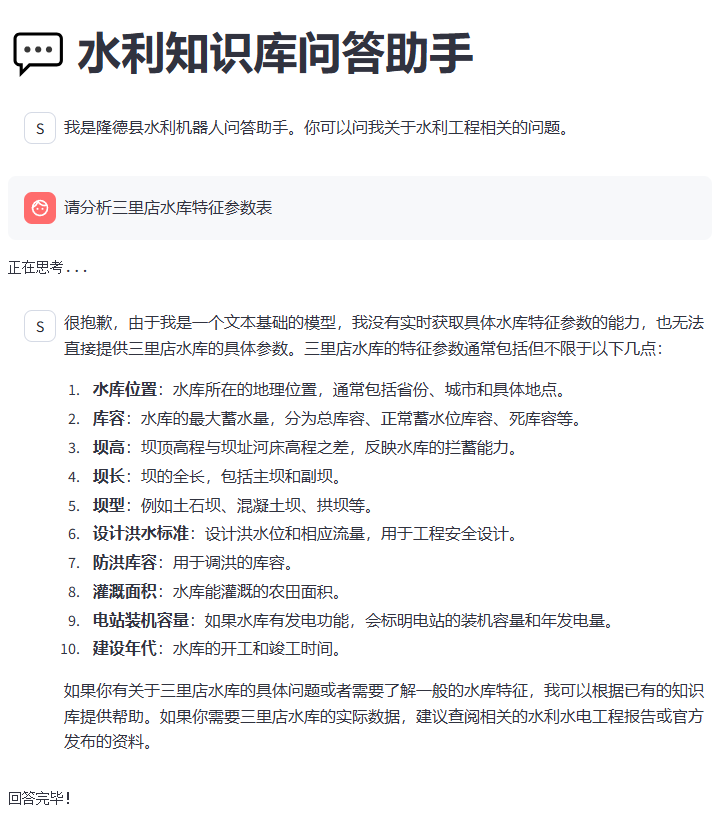
\includegraphics[width=0.8\textwidth]{无检索回答.png}
    \bicaption[无专业知识大模型回答]{无专业知识大模型回答}[Answer to the Large Model Without Professional Knowledge]{Answer to the Large Model Without Professional Knowledge}
    \label{fig:无检索}
\end{figure}
当面对特定的水利问题时,通用大模型通常无法提供准确的回答,这主要是由于其训练方式的局限性所致。此外,由于行业内封闭知识不对外公开,大模型无法通过常规训练途径获取这些知识。鉴于通过训练大模型来获得这些知识的计算成本和训练难度极高,因此选择将这些知识以提示词的形式输入大模型,以实现大模型对封闭领域知识的有效理解和应用。整体功能设计如图\ref{fig:rag整体结构图}所示。
\begin{figure}[h]
    \centering
    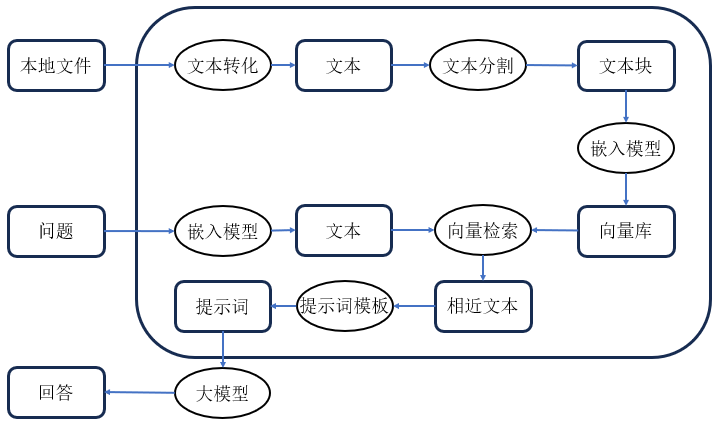
\includegraphics[width=0.75\textwidth]{rag整体结构图.png}
    \bicaption[RAG整体设计框架]{RAG整体设计框架}[Overall Design Framework of RAG]{Overall Design Framework of RAG}
    \label{fig:rag整体结构图}
\end{figure}
\subsection{向量数据库的构建}
在对水利局所辖的本地知识文件进行数据处理与分析过程中,发现其呈现出显著的格式异构性特征。具体而言,这些文件涵盖了多种不同类型的数据格式,包括Word文档、PDF文件、图像数据以及Excel表格等多元模态数据形式。针对其中的非结构化表格类文档,本研究采用了基于LangChain框架集成的OCR\cite{sarzynska2021detecting,tian2016detecting}(Optical Character Recognition,光学字符识别)文本提取接口,以实现对多模态数据的统一字符串转换,从而将图像中的文本信息以及其他非结构化数据转化为可处理的文本格式。

对于结构化表格文件的处理,则依据第四章所提出的结构化数据处理范式进行操作。其核心实现主要依赖于Python编程环境中的pandas数据分析库,通过该库强大的数据处理功能,能够有效地对结构化数据进行清洗、转换、分析以及可视化等操作,进而为后续的SQL生成与多级检索奠定坚实基础。
需特别指出的是,由于原始表格结构存在非规范化特征,许多文档在进行数据库转换时难以达到理想效果,如表\ref{tab:reservoir-scheduling}所示。即便数据以表格形式保存记录,但其内部缺乏多组信息之间的关联关系,本质上仅是利用部分表格结构来替代传统的文字叙述。

\begin{table}[htbp]
    \centering
    \bicaption[某水库部分调度计划表 ]{某水库部分调度计划表 }[Partial scheduling plan for a certain reservoir]{Partial Scheduling Plan for a Certain Reservoir}
    \label{tab:reservoir-scheduling}
    \begin{tabular}{|l|l|l|l|}
      \hline
      \multirow{6}{*}{泄水建筑物} & \multirow{3}{*}{开敞式溢洪道} & 型式 & 开敞式溢洪道 \\
      \cline{3-4}
      & & 进口高程(m) & 2061 \\
      \cline{3-4}
      & & 最大泄量(m³/s) & 114.9 \\
      \cline{2-4}
      & \multirow{2}{*}{最大泄量} & 断面尺寸(m) & 3.0×5.7 \\
      \cline{3-4}
      & & 最大泄量(m³/s) & 114.9 \\
      \hline
      \multirow{6}{*}{放水建筑物} & \multirow{3}{*}{水塔} & 型式 & 水塔 \\
      \cline{3-4}
      & & 闸门尺寸(m) & 1.0×1.0 \\
      \cline{3-4}
      & & 底坎高程(m) & 2051.7 \\
      \cline{2-4}
      & \multirow{3}{*}{涵管} & 断面尺寸(m) & 1.5×1.8 \\
      \cline{3-4}
      & & 最大泄量(m³/s) & 5.0 \\
      \cline{3-4}
      & & 最大泄量(m³/s) & 5.0 \\
      \hline
    \end{tabular}
  \end{table}
针对这种表格无法使用SQL来优化,但表格本身也不涉及到数学计算,表格长度较短,将这种表格称为结构化数据,通过JSON格式来增强文本结构化信息,如图\ref{fig:JSON}所示。形成由制表符文本到JSON再到database-SQL的三级存储形式。

\begin{figure}[!htb]
    \centering
    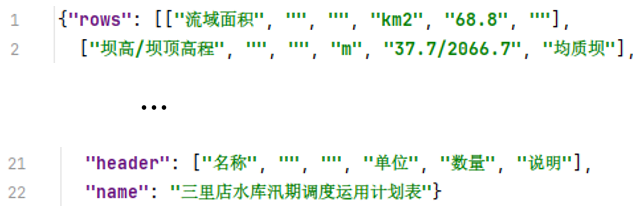
\includegraphics[width=0.8\textwidth]{json小.png}
    \bicaption[某水库部分调度计划表JSON格式]{某水库部分调度计划表JSON格式}[JSON form of Partial scheduling plan for a certain reservoir]{JSON Form of Partial Scheduling Plan for a Certain Reservoir}
    \label{fig:JSON} 
\end{figure}
\subsection{表格优化Agent设计}
在本研究构建的水利知识处理系统中,表格数据优化推理框架的流程图如图\ref{fig:SQL生成链}所示。该部分的核心功能在于:当本地知识召回的结果为表格文件时,利用第四章详细介绍的框架对召回的表格数据进行优化处理,并将优化后的表格数据输出给后续的流程,以供进一步的推理分析使用。这一过程对于确保数据的准确性和可用性至关重要,能够有效提升整个系统的推理分析效率和结果的可靠性。这部分是整个问答功能Langchain表达式的一部分。为了解问系统的整体设计与Langchain的配合,需要对Langchain的基本功能组成单元LangChain表达式(LangChain Expressions,LCEL)进行介绍。LCEL是 LangChain 框架中一种基本类,能够通过直观串行或并行的方式将各个功能组合,能够由众多可以实现子功能的基本LCEL以下成为子链(sub-chain)串连或并联组成具备完整功能的链(chain)而每一个子链是由Langchain最小组成单位runnable类构成。在本功能的具体实施过程中,构建了一个以用户问题作为输入参数,并以经过简化处理的表格数据作为输出结果的子链结构。
\begin{figure}[!htb]
    \centering
    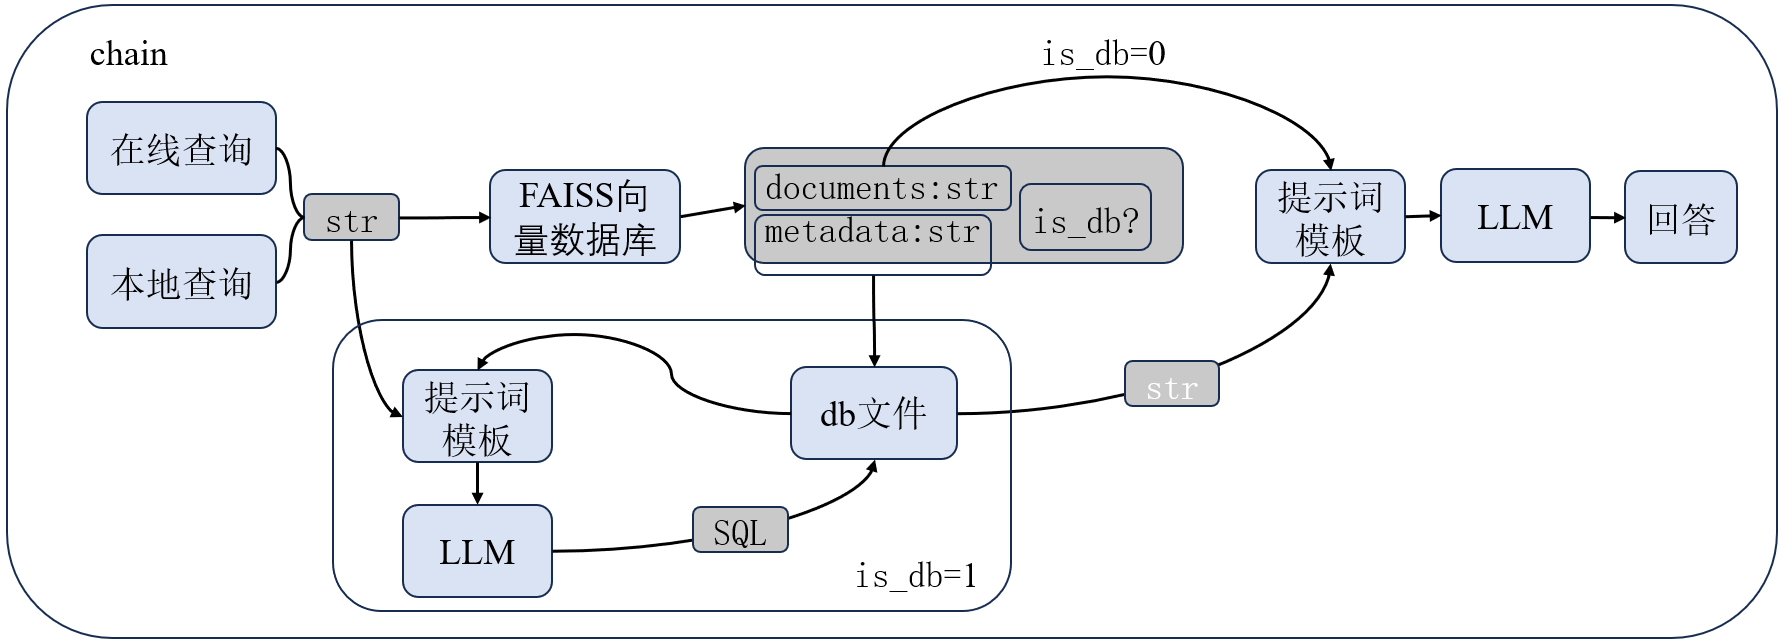
\includegraphics[width=0.9\textwidth]{SQL链生成示意图.png}
    \bicaption[SQL生成链示意图]{SQL生成链示意图}[SQL Generation Chain Diagram]{SQL Generation Chain Diagram}
    \label{fig:SQL生成链}
\end{figure}

在该子链的运行中,首先对 FAISS 向量数据库返回的 document 类别进行识别与处理。FAISS数据库进行两次检索,首先对向量库中的全部文本进行召回,此时使用的是文本相似度最邻近策略,将相似度最高的10个文本块(chunk)返回,在表格推理框架中则为10个表格文件,再由精排模型端到端地计算每个返回文本块与用户问题的相关性得分,取得分最高的文本块作为输出,当在本地环境中检测到第四章所介绍的三级存储结构时,系统会进一步判断是否可以采用 SQL 方法对表格进行优化。若判断结果为可行,则子链将生成相应的SQL语句并予以执行,随后将处理结果嵌入提示词模板,并输出给后续环节进行处理。反之,若判断结果为不可行,则子链将以结构化数据JSON的形式,将数据传递给后续环节,以确保数据的连续性和可用性。
\subsection{通用大模型推理功能设计}
在当前实现的功能中,问答功能主要基于单轮问答机制,即每次交互仅针对一个具体问题提供答案。然而,为了满足更复杂的对话需求,问答功能需要具备多轮问答功能。这要求系统能够记录上下文信息,以便在后续对话中引用历史内容。具体而言,历史对话以字典形式存储,其中包含三个关键字:“用户”(记录用户的提问)、“助手”(记录助手的回答)和“本地知识”(记录与对话相关的本地知识信息)。每轮对话的内容则以列表形式记录,以便于追踪对话的顺序和内容。

然而,在多轮对话和长文本检索的场景下,过长的上下文可能会对回答质量产生负面影响。这是因为新一轮对话未必与之前的每一轮对话及知识均存在关联性,过多的上下文信息可能会引入噪声,干扰模型的推理过程。为了解决这一问题,设计了一个子链结构,专门用于从历史上下文中检索与当前轮次对话相关的文本内容。该子链通过分析当前对话的主题和上下文,从历史记录中筛选出最相关的部分,从而确保模型在推理过程中仅参考有用的信息,提高回答的准确性和效率。这一机制的实现如图\ref{fig:多轮对话}所示,通过优化上下文管理,提升了多轮对话的整体性能。在上下文的文本检索过程中,为了提升系统的响应速度,仅采用单一的粗召回文本策略,并通过意图识别功能子链来判断在当前问答中是否需要在知识库中检索本地知识文档。

通过该子链,实际上将多轮问答任务转化为一种简化的形式,即通过提示词输入来替代传统的上下文传递方式,从而将多轮问答任务转化为单轮问答任务。这种设计既赋予了问答系统多轮问答的能力,使其能够理解和处理多轮对话中的上下文信息,又保持了单轮问答任务在计算成本和推理难度方面的优势,降低了系统的复杂性和资源消耗。

\begin{figure}[!htb]
    \centering
    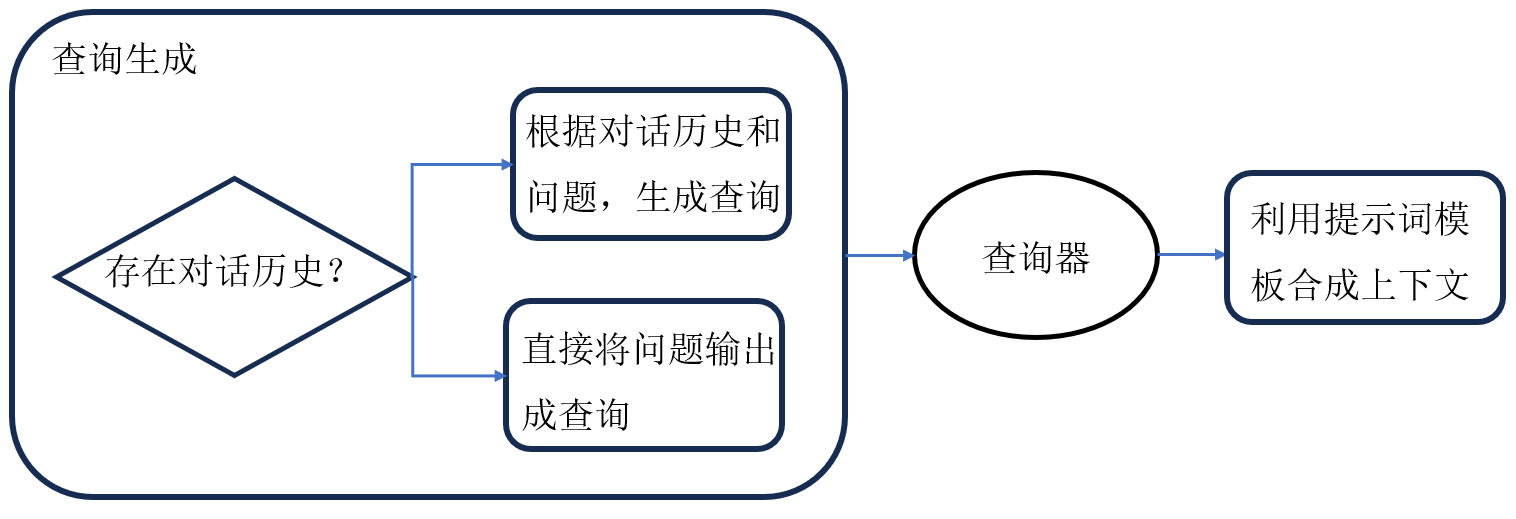
\includegraphics[width=0.88\textwidth]{对话历史生成流程图.png}
    \bicaption[对话历史生成流程图]{对话历史生成流程图}[Chat History Generation Flowchart]{Chat History Generation Flowchart}
    \label{fig:多轮对话}
\end{figure}
特别是对于直接将输出反馈给用户的环节,会将大模型的输出方式设置为流式输出(stream),即大模型的输出采用流式输出而非一次性输出所有答案,主要原因在于:一方面,流式输出能够逐步返回生成的中间结果,使用户能够更早地看到部分答案,减少等待时间,从而提升用户体验,增强交互的实时性和流畅性;另一方面,对于长时间的生成任务,一次性存储完整的输出会占用大量内存,而流式输出可以逐块返回结果,避免了一次性存储大量数据,从而降低内存占用。此外,流式输出能够适应实时应用需求,提供更自然的交互体验;同时,当输出内容较长时,一次性传输可能会导致请求超时,而流式输出可以分批次发送数据,降低超时风险,确保数据传输的稳定性。流式输出还可以模拟真实对话的输出节奏,让用户在AI生成回答时就能开始阅读,提前思考或及时打断对话,使交互过程更加流畅自然。

\section{知识库功能设计}

本小节希望通过建立业务规则库来支撑业务场景的规则适配,规范和约束水利业务管理行为,并同时以向量数据库的形式存储,为大模型问答功能提供知识,如图\ref{fig:知识库流程图}。
\begin{figure}[htbp]
    \centering
    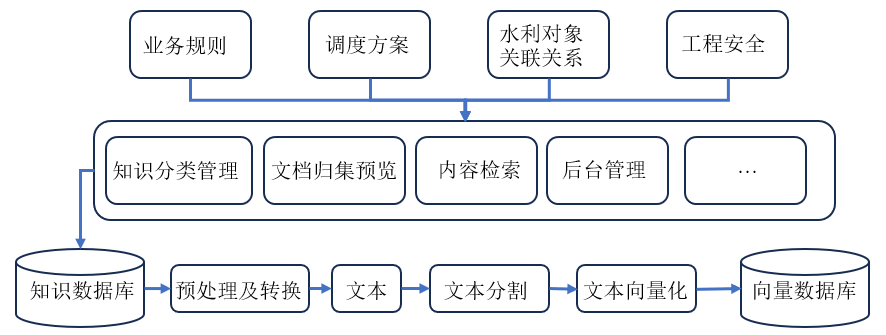
\includegraphics[width=0.9\textwidth]{知识库流程图.png}
    \bicaption[知识库流程图]{知识库流程图}[Knowledge Base Process Diagram]{Knowledge Base Process Diagram}
    \label{fig:知识库流程图}
\end{figure}
\begin{table}[htbp]
    \centering
    \renewcommand{\arraystretch}{1.2} % 调整行距
    \begin{minipage}[t]{0.8\linewidth}
        \bicaption[功能说明]{功能说明}[Function Description]{Function Description}
        \label{tab:功能说明}
        \begin{tabularx}{\linewidth}{l>{\centering\arraybackslash}X}
            \toprule[1.5pt]
            {\heiti 功能} & {\heiti 说明} \\
            \midrule[1pt]
      文档分类 & 对所有的文档进行分类,分类分级,在首页中可选择不同的分类查询对应的文档。 \\
      
      文档检索 & 提供强大的检索功能,支持全文检索、关键词检索、分类检索等多种检索方式,帮助用户快速找到所需文档。 \\
      
      文档下载 & 用户可以下载权限范围内的知识文档。 \\
      
      在线预览 & 对已经上传的文档在线预览,文件格式包括:.doc, .docx, .rtf, .odt, .dot, .fdf, .ppt, .pttx, .xls, .xltx, .csv, .chm, .txt, .pdf, .html。 \\
      
      文档管理 & 管理员可以对文档内容、类别、版本、属性、标签和权限进行修改和维护。 \\
      
      存储管理 & 提供安全、可靠的存储空间,用于存放知识库中的各类文件,如文本、图片、视频、音频等。 \\
      
      目录管理 & 根据知识库的内容和分类方式,设计合理的目录结构,包括一级目录、二级目录等,以便将知识内容进行归纳和整理。 \\
      
      标签管理 & 给知识添加标签,可以为其关联关键词或主题,便于用户快速筛选和查找相关内容。 \\
      \bottomrule[1.5pt]
    \end{tabularx}
\end{minipage}
\end{table}
调度方案库包括旱灾防御、水资源调度和管网爆漏应急等预案,并将调度预案进行分类保存;建立水利对象关联关系文档库,进行结构化分类和关联,便于水利知识的快速检索和定位;建立工程安全知识库,为工程安全管理提供知识服务,提高工程安全管理决策水平。
知识库文件管理功能主要包括以下几个方面:
1. 知识库分类与分级:对知识库进行分类和分级管理,便于用户根据需求快速
定位和查找相关知识文件。分类包括预报调度方案库、工程安全知识库、业务规则库
等,各分类下可分为不同级别。
2. 知识库文档管理:系统管理员可对文档进行维护上传、分类维护等操作,确
保知识库内容的完整性和准确性。
3. 知识库文件检索:提供模糊搜索功能,用户可通过关键词、文档标题、上传
日期等信息在知识库中快速检索所需知识文件。
4. 知识库文件在线预览与下载:支持多种文件格式的在线预览,如.doc、.ppt、.xls等。用户可在线预览文件,并根据需要进行下载。其他具体功能如表\ref{tab:功能说明}所示,图\ref{fig:知识库管理}为知识库的前端界面。
\begin{figure}[htbp]
    \centering
    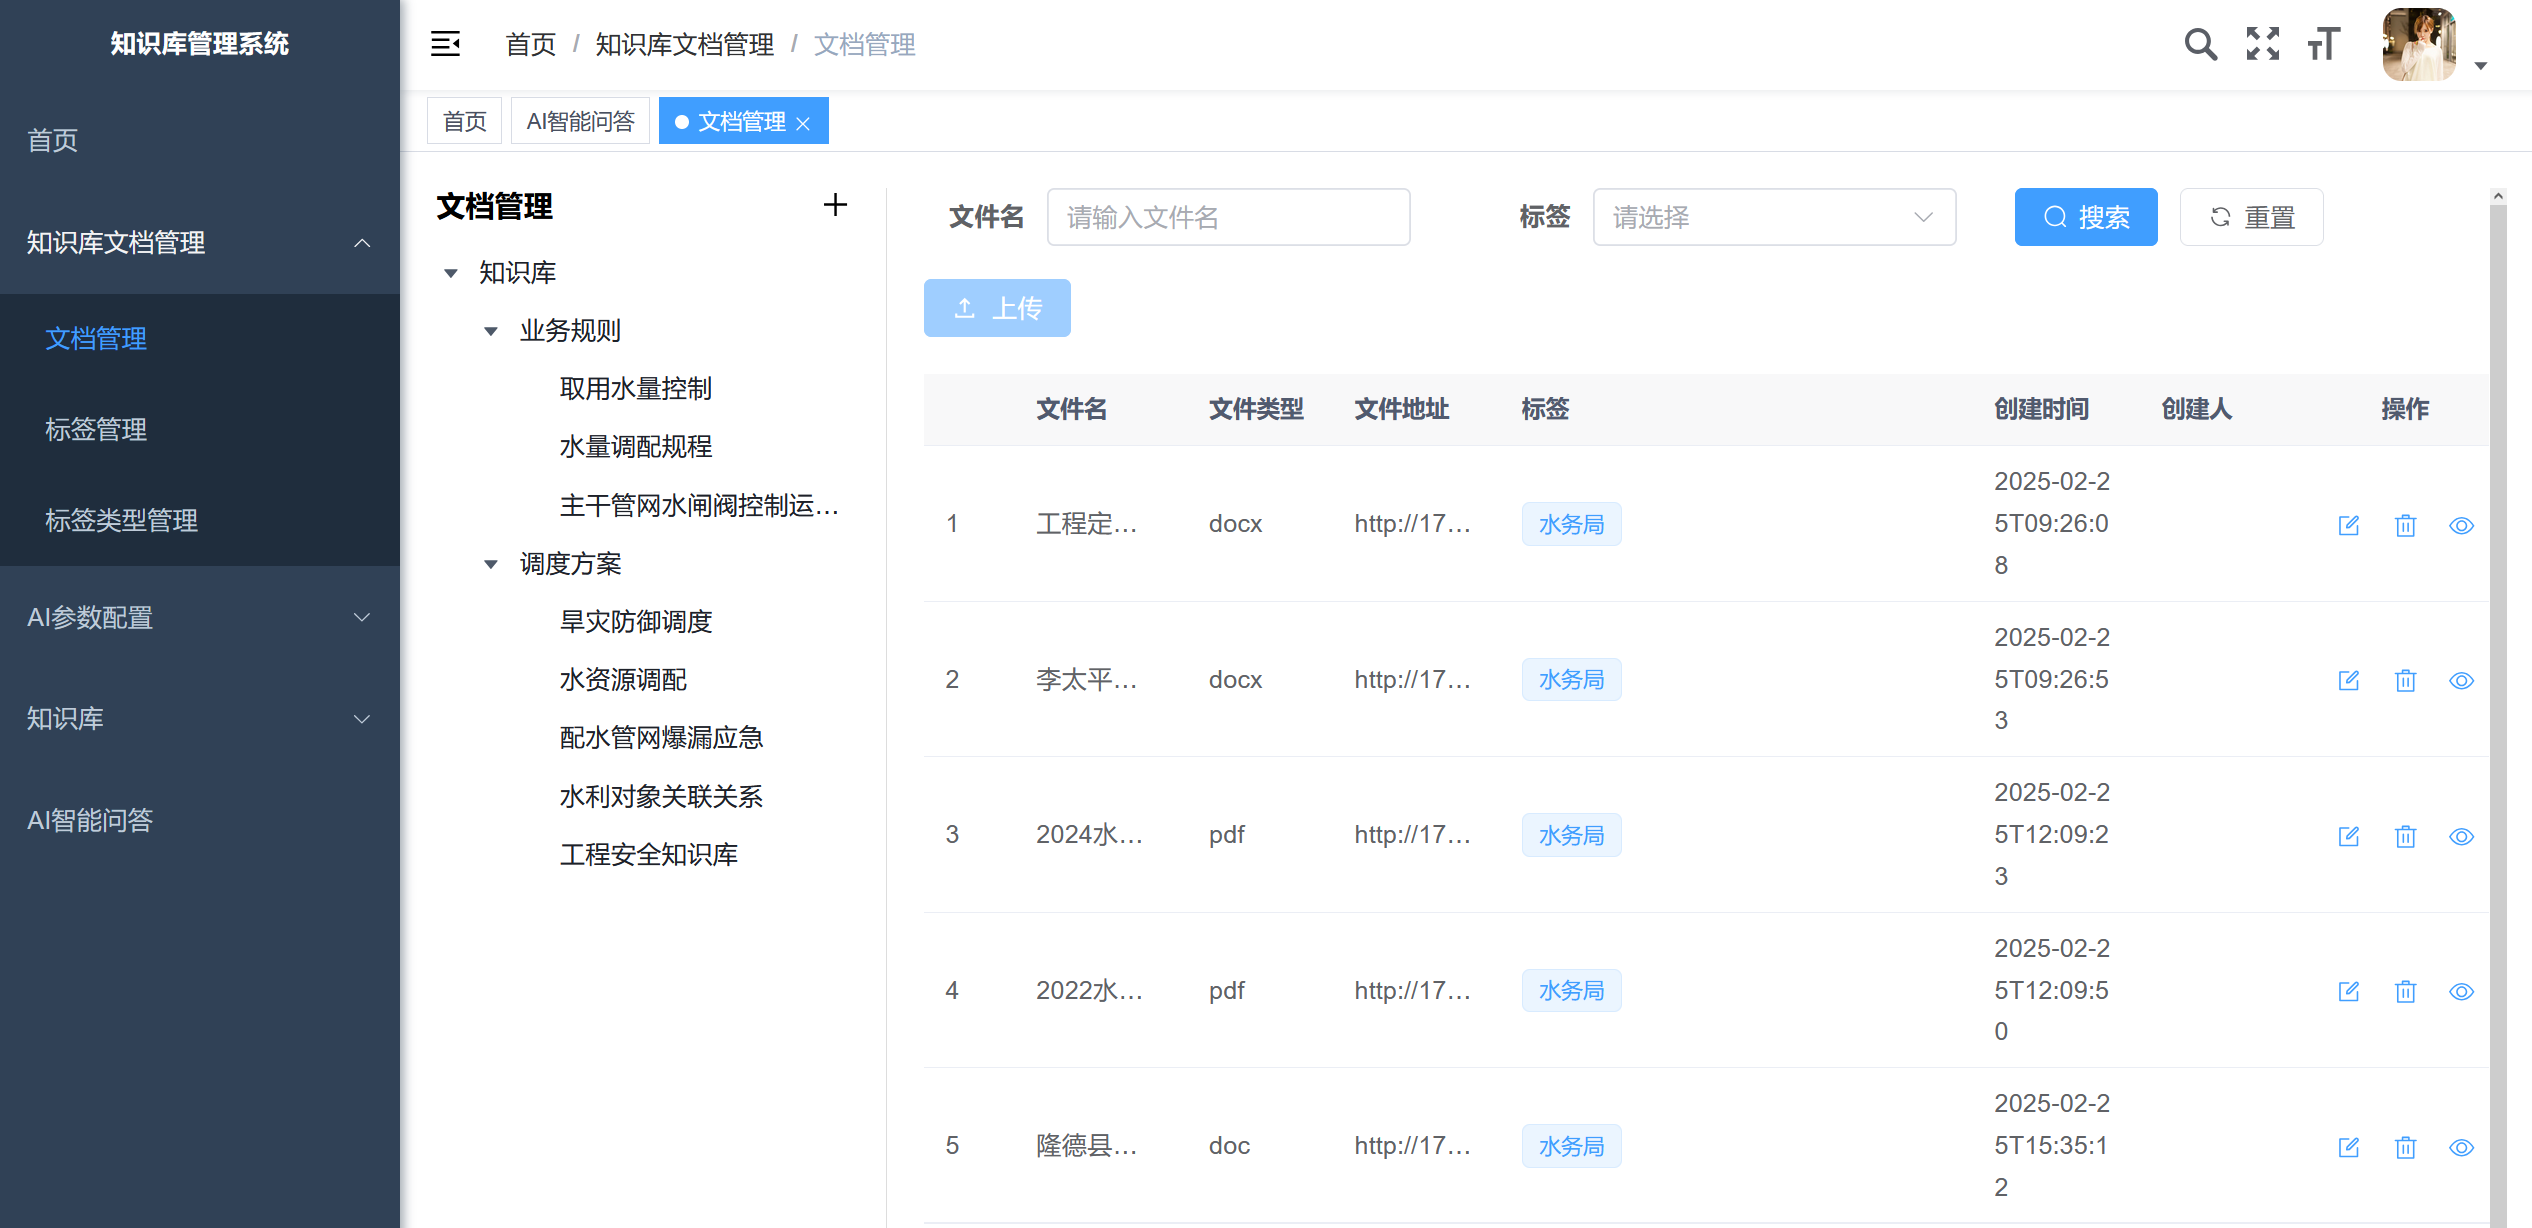
\includegraphics[width=0.91\textwidth]{知识库管理界面.png}
    \bicaption[知识库管理界面]{知识库管理界面}[Knowledge base management interface]{Knowledge Base Management Interface}
    \label{fig:知识库管理}
\end{figure}
\begin{figure}[!htbp]
    \centering
    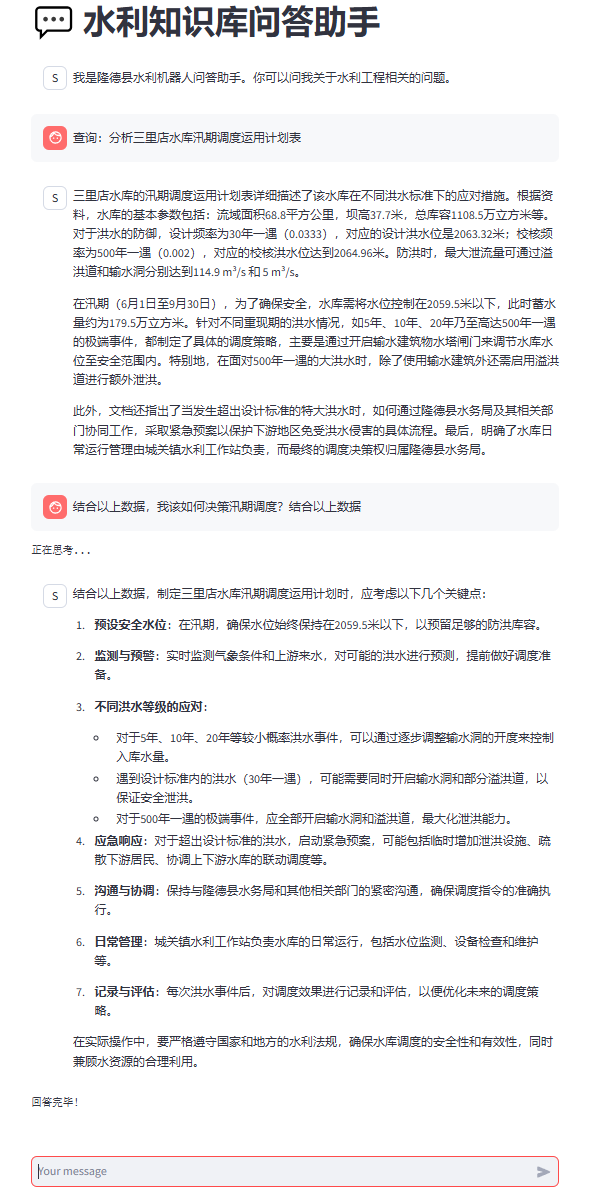
\includegraphics[width=0.75\textwidth]{多轮回答.png}
    \bicaption[多轮问答功能]{多轮问答功能}[ Multi round Q\&A function]{ Multi Round Q\&A Function}
    \label{fig:多轮对话展示}
\end{figure}

下面通过图\ref{fig:单轮问答}、图\ref{fig:结构化数据}和图\ref{fig:多轮对话展示}展示了表格数据推理框架在实际应用中的对话效果以及针对知识库的智能问答系统的界面展示。其中,图\ref{fig:单轮问答}呈现了表格的单轮问答效果,当系统识别到表格信息时,会将Agent输出的database表格展示在界面中,并支持对展示表格的保存功能。图\ref{fig:多轮对话展示}则展示了在多轮对话场景下系统的推理结果,这些结果由通用大模型根据上下文中的本地知识进行分析后生成。图\ref{fig:结构化数据}展示了当检索返回的表格为结构化数据表格时的推理结果,从回答中可以看出,大模型对JSON形式的结构化数据具备良好的推理能力。

\begin{figure}[htb]
    \centering
    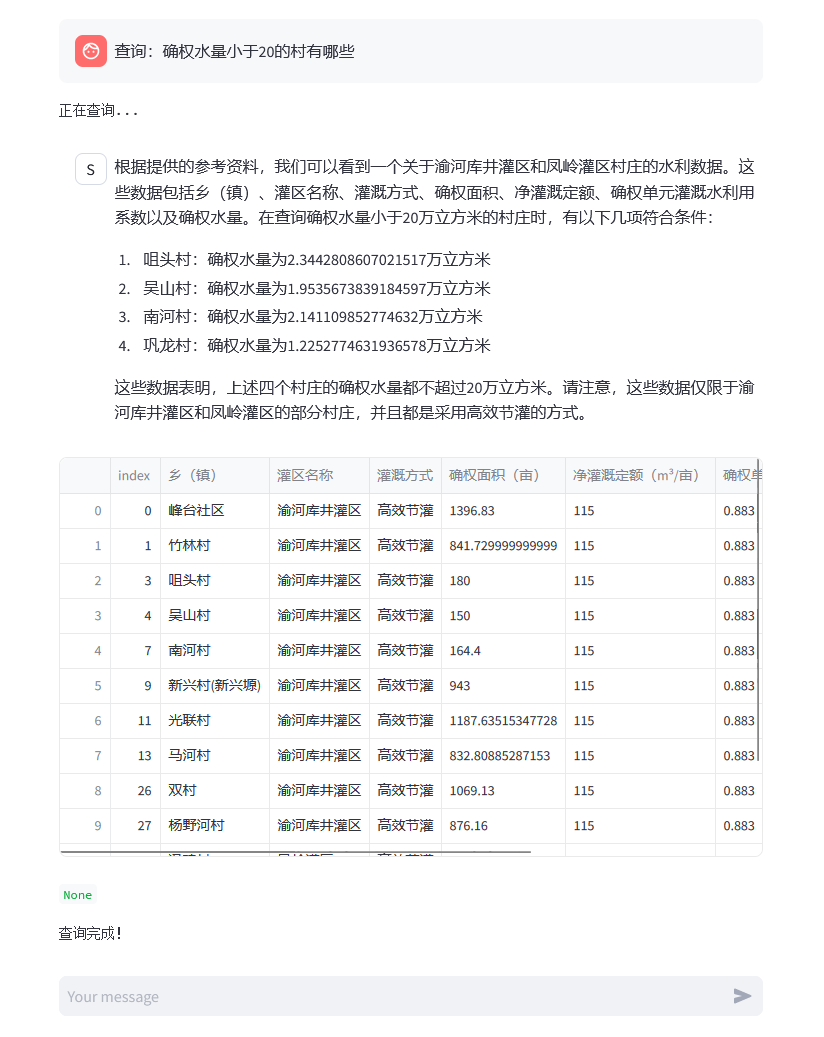
\includegraphics[width=0.82\textwidth]{单轮问答表格推理.png}
    \bicaption[单轮问答表格推理]{单轮问答表格推理}[Offline Database File Upload Function]{Offline Database File Upload Function}
    \label{fig:单轮问答}
\end{figure}
% 在单轮的查询过程中,反馈系统会将全部符合条件的表格数据返回给用户,并通过表格展示的方式,将表格数据以可视化的形式展示给用户。用户可以通过点击表格中的链接,查看表格的详细内容。同时对表格内容含义等相关信息进行解释说明。
% 在多轮对话的过程中,反馈系统会根据用户的提问,从上下文和知识库中检索需要信息进行进一步推理,提出更准确的专家意见与决策,生成更高质量的回答。
在智能问答系统中,单轮查询与多轮对话是两种主要的交互模式。在单轮查询过程中,问答系统将符合查询条件的所有表格数据完整地返回给用户。为了增强数据的可读性与用户体验,系统采用表格展示的方式,将数据以结构化的形式呈现,使用户能够清晰地浏览各项信息。此外,为了满足用户深入了解数据的需求,表格中的特定元素被设计为可点击的链接。用户通过点击这些链接,可以将召回的表格以excel格式下载保存,从而获取表格中各项数据的详细内容。系统还配备了相应的解释说明功能,对表格中数据的含义、背景以及相关关联信息进行解读,帮助用户全面理解数据所传达的信息。
而在多轮对话场景下,问答系统则需要具备更强的逻辑推理与信息整合能力。随着对话的深入,用户的问题往往更加复杂且具有上下文依赖性。此时,问答系统不仅要关注当前提问,还需将之前的对话内容作为重要的参考依据,同时深度挖掘知识库中的相关知识,通过复杂的语义分析与逻辑推理,将新获取的信息与已有信息进行融合,从而提出更加精准、更具专业性的专家意见与决策建议。
\begin{figure}[ht]
    \centering
    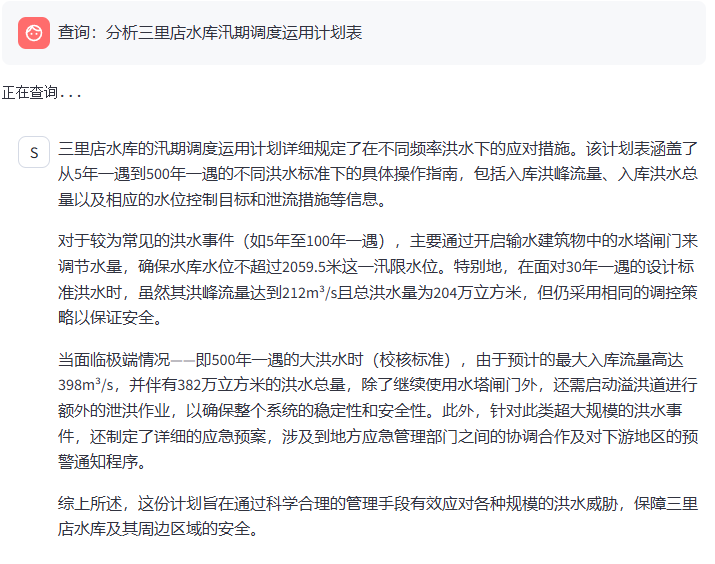
\includegraphics[width=0.74\textwidth]{结构化数据处理功能.png}
    \bicaption[结构化数据处理功能]{结构化数据处理功能}[Structured data processing function]{Structured Data Processing Function}
    \label{fig:结构化数据}
\end{figure}


\section{本章小结}
% 本章聚焦于第前两章提出的技术在水利领域智能问答系统中的应用。
本章聚焦于RAG系统在智能问答助手中的应用研究。
系统关键技术框架构建方面,基于LangChain框架与FAISS向量数据库,设计并实现了高效的检索增强生成(RAG)问答系统。通过整合多级表格数据检索、大模型推理优化及用户交互界面,构建了完整的端到端技术链路,显著提升了系统对结构化数据的处理能力与响应效率。RAG问答功能优化方面,针对水利领域专业知识的封闭性与复杂性,提出多级表格数据检索方法,通过表头与表名的向量化存储策略,解决了传统文本切块导致的表格信息失真问题。结合循环推理框架与Agent代理思想,将复杂表格任务分解为SQL生成与执行的多步流程,有效弥补了大模型在数值推理与长上下文处理中的局限性,提升了回答的准确性。

知识库管理功能实现方面,设计并开发了知识库的动态管理功能,支持用户对本地文件的查询和浏览。通过JSON与SQLite的三级存储结构,实现了结构化表格数据的高效存储与快速检索,确保系统在水利调度场景下的灵活性与可扩展性。实际应用与效果验证方面,通过实际案例展示了系统在单轮问答、多轮对话及结构化数据处理中的表现。实验结果表明,问答系统能够准确召回本地知识、生成专业建议,并通过流式输出与交互式界面优化用户体验,为水利从业人员提供了高效、可靠的技术支持。本章内容不仅验证了检索增强生成技术与Agent框架在垂直领域中的实用价值,也为后续智能化问答系统的设计与行业落地提供了重要参考。

本章主要内容以作者在合作企业进行实习期间所撰写的实习报告形式提交,该知识库的智能问答系统已在隆德县水利局正式上线并投入使用。
